
\eucommentary{Please provide the following:\\
\begin{compactitem}
\item
brief presentation of the overall structure of the work plan;
\item
timing of the different work packages and their components (Gantt chart or similar);
\item
detailed work description, i.e.:
\begin{compactitem}
\item
a description of each work package (table 3.1a);
\item
a list of work packages (table 3.1b);
\item
a list of major deliverables (table 3.1c);
\end{compactitem}
\item
graphical presentation of the components showing how they inter-relate (Pert chart or similar).
\end{compactitem}
}

\subsubsection{Overall Structure of the Work Plan}\label{sec:workplan-structure}

\ifgrantagreement
The
\else
As shown in Table~\ref{fig:wplist}, the
\fi
work plan is broken down into
six work packages:
\WPref{core} about maintaining the core Jupyter software infrastructure,
\WPref{ecosystem} for developing the ecosystem of software surrounding Jupyter,
\WPref{applications} for building applications to demonstrate the efficacy and guide the development
of core infrastructure,
\WPref{eosc} for operating services built on these
components and collaborating with existing EOSC stakeholders,
\WPref{education} for educating the public on Open Science best practices with the project's tools
and fostering diversity in the research and software communities.
This is complemented by
the usual management  work package
(\WPref{management}). The Gantt chart on
Page~\pageref{fig:gantt} illustrates the timeline for the various
tasks for these work packages.
%, including inter-task dependencies.

\ifgrantagreement\else
%\makeatletter\wp@total@RM{management}\makeatother
\wpfigstyle{\footnotesize\def\tabcolsep{3.5pt}}
%\wpfig[pages,type,start,end]
{\wpfig}
\fi

\begin{figure}[htb]
  \centering
  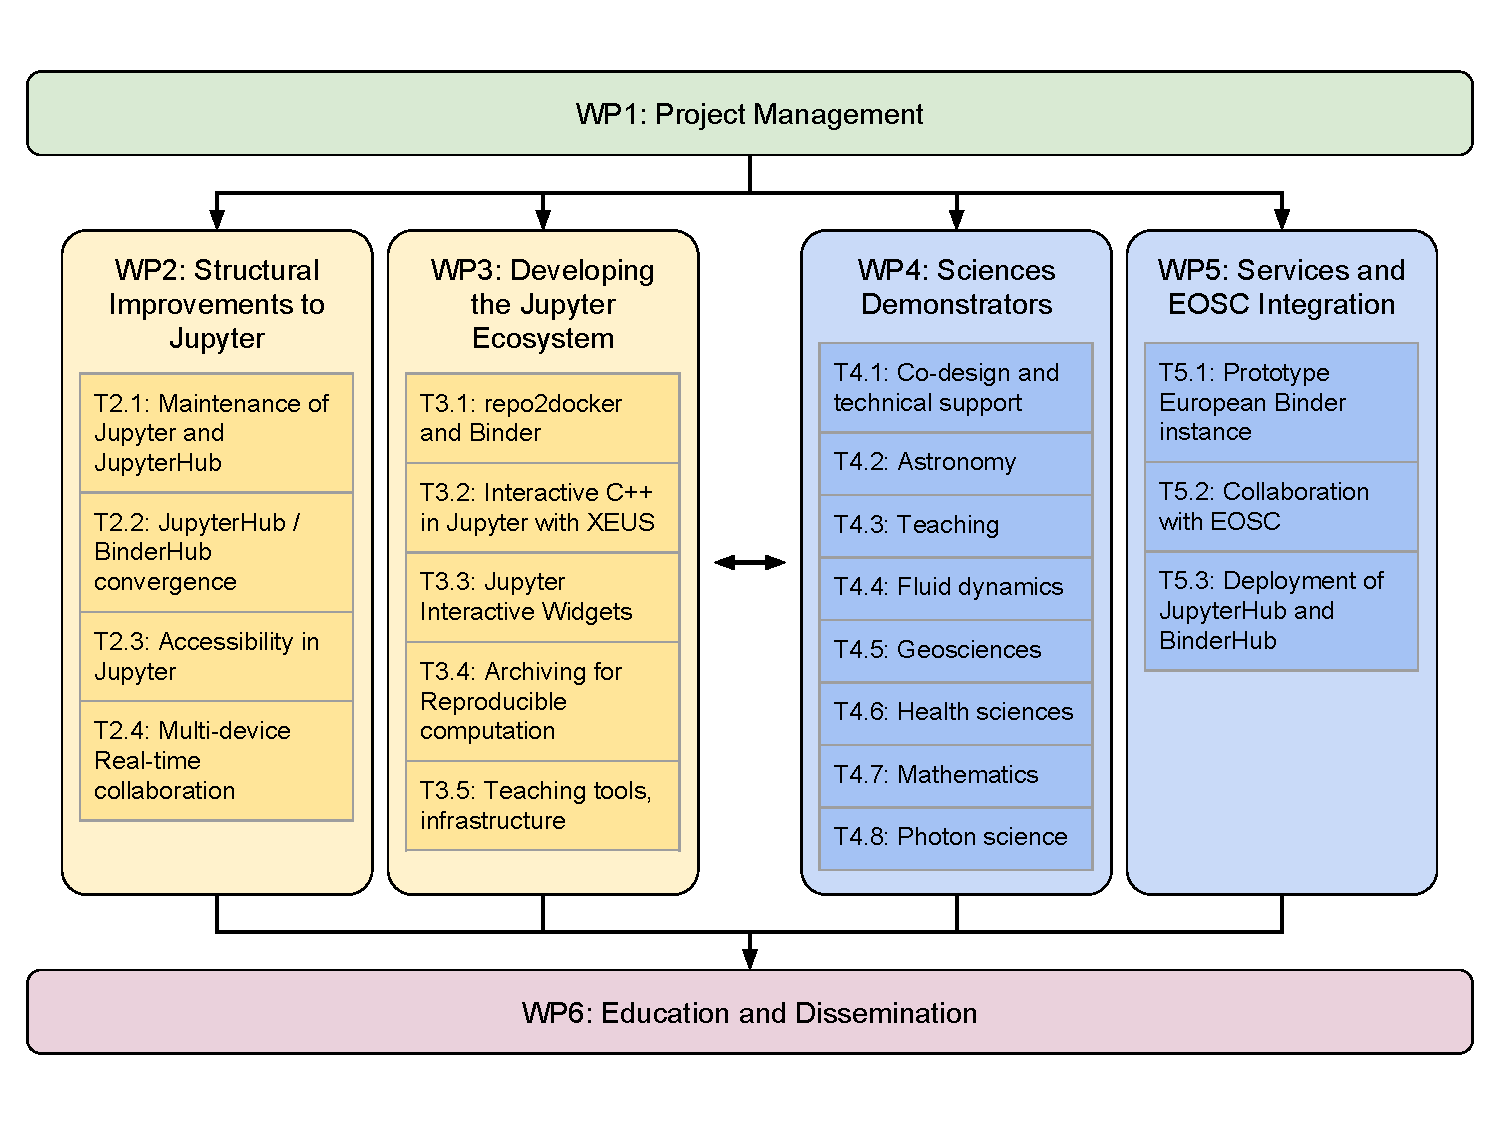
\includegraphics[width=0.9\textwidth]{images/workpackages.pdf}
  \caption{
    \label{fig:workpackages}
    The relationships and interactions of the work packages,
    broken up into four main categories: Management (WP1),
    Development of new functionality surrounding Jupyter (WP2, WP3),
    Demonstrators and Services (WP4, WP5),
    and Education and Dissemination (WP6).
    Ultimately, all work packages benefit from and feed back to
    all other work packages.
  }
\end{figure}

% \subsubsection{How the Work Packages will Achieve the Project Objectives}
% \label{sssec:how_the_work_packages_will_achieve}

\gantttaskchart[draft,xscale=.33,yscale=.33,milestones]

\ifgrantagreement\else
\newpage
\subsubsection{Deliverables}\label{sec:deliverables}
\inputdelivs{9.3cm}
\fi

\newpage
\subsubsection{Milestones}\label{sec:milestones}
\eucommentary{Milestones means control points in the project that help to chart progress. Milestones may
correspond to the completion of a key deliverable, allowing the next phase of the work to begin.
They may also be needed at intermediary points so that, if problems have arisen, corrective
measures can be taken. A milestone may be a critical decision point in the project where, for
example, the consortium must decide which of several technologies to adopt for further
development.}



\paragraph{General Milestones}

\begin{milestones}
  \milestone[
    id=startup,
    month=12,
    verif={
      Completed all corresponding deliverables
      and preparation for deployment of prototype services is underway
      }
    ]
  {Startup}
  {
  By milestone 1, we will have established the infrastructure
  for the project and begun prototyping development,
  engaging with the existing communities,
  coordinating plans for \TheProject with those of the wider Jupyter and open science communities.
  EGI Infrastructure-as-a-Service (IaaS) cloud resources are available with a
  Service Level Agreement (SLA) for \TheProject,
  and
  }

  \milestone[
    id=prototype,
    month=24,
    verif={
      Completed all corresponding deliverables and early users are able to access and test prototype services
    }
    ]
  {Working prototypes}
  {
  By milestone 2, we will have working prototypes of services
  for open science, and begun to experiment with early-adopter
  users to guide further development of \TheProject,
  ensuring that development serves the needs of the community.
  An initial \TheProject Service Management System shall be available,
  and \TheProject services are integrated with the EOSC Marketplace,
  and AAI Cloud services.
  }

  \milestone[
    id=community,
    month=36,
    verif={Completed all corresponding deliverables and services
    are operational and ready for public testing}
    ]
  {Community engagement}
  {
  By milestone 3, services should be useful and accessible
  to a broad range of users.
  By this point, we will have training materials and run
  workshops to train users in Open Science,
  gathering feedback to guide the further development of \TheProject.
  \TheProject Service Management System is fully compliant with the EOSC Service Management practices
  }


  \milestone[
    id=final,
    month=48,
    verif={Completed all corresponding deliverables and reported progress at the final project review}
  ]
  {Adoption and sustainability}
  {
  By this point, all \TheProject services should be operational, TRL 8.
  Through community engagement via workshops, conferences, and other media,
  the services should have established groups of users,
  benefiting from these services and improving the Open Science landscape
  on EOSC and beyond.
  }

\end{milestones}


% ---------------------------------------------------------------------------
% Include Work package descriptions
% ---------------------------------------------------------------------------

\input{WorkPackages/WorkPackages}


%%% Local Variables:
%%% mode: latex
%%% TeX-master: "proposal"
%%% End:
